
%%%% Réalisation de la page de garde

\begin{titlepage}
\begin{center}
%\flushleft

\includegraphics[height=30mm,width=30mm]{logo.jpg} %insérer un dessin
\hfill%
%\hspace*{10,5cm}
%\includegraphics[height=30mm,width=30mm]{logo_gbi.jpg}\\
%\begin{center}
%\centering
%\includegraphics[height=20mm,width=20mm]{institut_limerick.jpg}
%\hspace*{1cm}
%\flushright

\includegraphics[height=40mm,width=20mm]{logo_sfa.jpg}\\
\end{center}
\vspace*{1cm}



%%%%%%%%%%%%%%%%%%% Déclaration du type de document%%%%%%%%%%%%%%%%%%%%%%%%%
\begin{center}
\textsc{Universit\'e de Poitiers,}\paragraph{}
 Master 1 Réseaux Télécommunications Multimédia et Automatique
\end{center}


\begin{center}
\texttt{Compte rendu de Travaux pratiques\\ Système de Transmission Multimedia}\\
\texttt{Du 26 Mars au 14 Avril 2015} %textcolor c est pour mettre la couleur 
\end{center}
\vspace*{2cm}
 



%\textsc{Universit\'e de Poitiers, M1 RTMA} \\ %[25pt] % Your university, school and/or department name(s)
%\horrule{0.5pt} \\[0.4cm] % Thin top horizontal rule
%\huge {\color{blue}Travaux pratiques en Méthodes statistiques}  % Title

%\author{Guy-Florent \textsc{Sadeler}, \\Thomas \textsc{Le Bris}.} % Author name

%\date{\today} % Date for the report \date{\normalsize\today} % Today's date or a custom date 
 
 
\begin{center}
%\begin{framed}
% Commande permettant de définir l'écart
\setlength{\fboxsep}{2mm}
% Commande permettant de définir l'épaisseur du trait
\setlength{\fboxrule}{2mm}
\fbox{\textcolor{blue}{{{\textbf{\textit{\fontfamily{pnc}\selectfont{Transmission Multimedia sur canaux extrêmement sensibles (Qualité et sécurité)}}}}}}}%textsc utiliser pour petite majuscule, \selectfont	active la police définie
%\end{framed}
\end{center}

\vspace*{1.5cm}
\begin{center}
\begin {figure}[htbp]
  \hbox{ 
     
\includegraphics[height=50mm,width=70mm]{intro2}%[width=5cm][scale=0.45]
     \hspace*{1cm}  %% pour mettre un espace (horizontal) de 5cm entre les deux images
     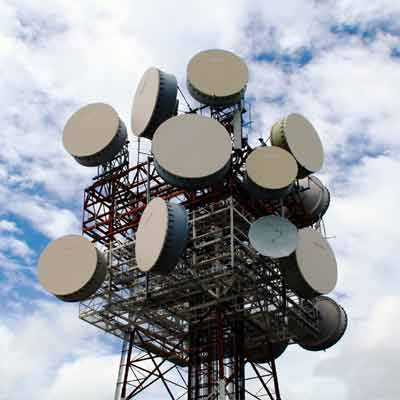
\includegraphics[height=50mm,width=70mm]{tel}
  }
\end {figure}
\end{center}


\vspace*{1cm}

%\par \vspace{2cm}
%\begin{center}
%\includegraphics[height=60mm,width=60mm]{gaussienne.jpg}
%\end{center}
%\par \vspace{2cm}


  % emphasize mettre l'accent sur le texte mis en accolade
 %textbf pour mettre le texte en gras 


\begin{center}
\begin{tabular}{l r}

Groupe d'étudiants: & \texttt{Guy-Florent \textsc{Sadeler} }\\ % Partner names
&  \texttt{Thomas \textsc{Le Bris}}

\end{tabular}
\end{center}

\vspace*{1cm}
\begin{center}
\begin{tabular}{l r}
Responsable pédagogique: & \texttt{Clency \textsc{Perrine}} % Instructor/supervisor
\end{tabular}
\end{center}




\end{titlepage}